%!TEX root = ../Main.tex


\begin{figure}
% \Large
% \begin{dot2tex}[scale=0.5]
% digraph {
%     rankdir=LR;
%     mindist=0.1
%     nodesep=0.1;
%     ranksep=0.1;
%     node [shape="circle", margin=0];
%     10 [label="Pull xs"];
%     20 [label="Out o (f x)"];
%     30 [label="Release x"];
% 
%     90 [label="OutDone o"];
%     91 [label="Done"];
% 
%     10 -> 20 [label="Some x"];
%     10 -> 90 [label="None"];
% 
%     90 -> 91;
% 
%     20 -> 30;
%     30 -> 10;
% }
% \end{dot2tex}

\centering
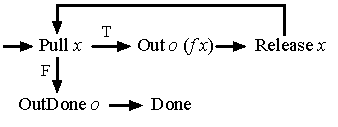
\includegraphics{machine/map}
\caption{$os =$~map~$f$~$xs$}
\label{fig:com:map}
\end{figure}

\begin{figure}
%\Large
%\begin{dot2tex}[scale=0.5]
%digraph {
%    rankdir=LR;
%    mindist=0.1
%    nodesep=0.1;
%    ranksep=0.1;
%    node [shape="circle", margin=0];
%    10 [label="Pull xs"];
%    15 [label="If (p x)"];
%    20 [label="Out o x"];
%    30 [label="Release x"];
%
%    90 [label="OutDone o"];
%    91 [label="Done"];
%
%    10 -> 15 [label="Some x"];
%    15 -> 20 [label="True"];
%    15 -> 30 [label="False"];
%    10 -> 90 [label="None"];
%
%    90 -> 91;
%
%    20 -> 30;
%    30 -> 10;
%}
%\end{dot2tex}

\centering
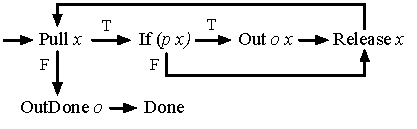
\includegraphics{machine/filter}
\caption{$os =$~filter~$p$~$xs$}
\label{fig:com:filter}
\end{figure}

\begin{figure}
%\Large
%\begin{dot2tex}[scale=0.5]
%digraph {
%    rankdir=LR;
%    mindist=0.1
%    nodesep=0.1;
%    ranksep=0.1;
%    node [shape="circle", margin=0];
%    10 [label="Pull xs"];
%    11 [label="Pull ys"];
%    20 [label="Out o (x,y)"];
%    30 [label="Release x"];
%    31 [label="Release y"];
%
%    80 [label="Close ys"];
%    88 [label="Close xs"];
%    89 [label="Release x"];
%
%    90 [label="OutDone o"];
%    91 [label="Done"];
%
%    10 -> 11 [label="Some x"];
%    11 -> 20 [label="Some y"];
%    10 -> 80 [label="None"];
%    80 -> 90;
%    11 -> 88 [label="None"];
%    88 -> 89;
%
%    89 -> 90;
%
%    90 -> 91;
%
%    20 -> 30;
%    30 -> 31;
%    31 -> 10;
%}
%\end{dot2tex}

\centering
\hspace{-3ex}
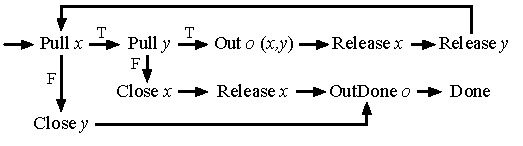
\includegraphics{machine/zip}
\caption{$os =$~zip~$xs$~$ys$}
\label{fig:com:zip}
\end{figure}


\begin{figure*}
%\Large
%\begin{dot2tex}[scale=0.45]
%digraph {
%    rankdir=LR;
%    mindist=0.0
%    nodesep=0.0;
%    ranksep=0.4;
%    node [shape="circle", margin=0];
%
%    10 [label="Pull xs"];
%    20 [label="Pull ys"];
%    30 [label="If (x le y)"];
%
%    40 [label="Out o x"];
%    41 [label="Release x"];
%    42 [label="Pull xs"];
%
%    50 [label="Out o y"];
%    51 [label="Release y"];
%    52 [label="Pull ys"];
%
%    100 [label="Pull ys"];
%    101 [label="Out o y"];
%    102 [label="Release y"];
%
%    200 [label="Pull xs"];
%    201 [label="Out o x"];
%    202 [label="Release x"];
%
%    900 [label="OutDone o"];
%    901 [label="Done"];
%
%    10 -> 20 [label="Some x"];
%    10 -> 100 [label="None"];
%    20 -> 30 [label="Some y"];
%    20 -> 201 [label="None"];
%
%    30 -> 40 [label="True"];
%    30 -> 50 [label="False"];
%
%    40 -> 41;
%    41 -> 42;
%
%    42 -> 30 [label="Some x"];
%    42 -> 101 [label="None"];
%
%    50 -> 51;
%    51 -> 52;
%    52 -> 30 [label="Some y"];
%    52 -> 201 [label="None"];
%
%    100 -> 101 [label="Some y"];
%    100 -> 900 [label="None"];
%    101 -> 102;
%    102 -> 100;
%
%    200 -> 201 [label="Some x"];
%    200 -> 900 [label="None"];
%
%    201 -> 202;
%    202 -> 200;
%
%    900 -> 901;
%}
%\end{dot2tex}

\centering
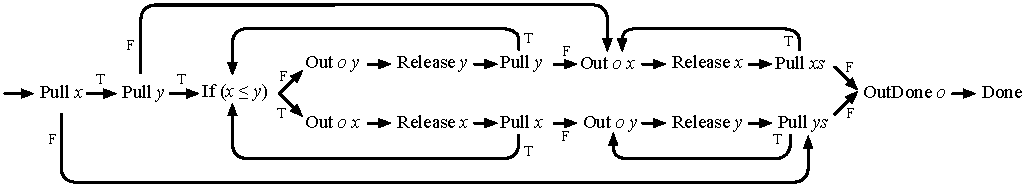
\includegraphics{machine/merge}
\caption{$o =$~merge~$xs$~$ys$}
\label{fig:com:merge}
\end{figure*}


\begin{figure}
{ \centering
\Large
\begin{dot2tex}[scale=0.35]
digraph {
    rankdir=LR;
    mindist=0.1
    nodesep=0.1;
    ranksep=0.1;
    node [shape="circle", margin=0];
    0 [label="Pull xs (init)"];
    1 [label="Update o_s = xs"];
    2 [label="Release xs"];
    3 [label="Pull xs"];

    4 [label="If eqfst"];

    10 [label="Update o_s = update"];

    20 [label="Out o_s"];

    30 [label="Out o_s"];

    40 [label="OutDone o"];

    50 [label="Done"];

    0 -> 1 [label="Some"];
    0 -> 40 [label="None"];
    2 -> 3;
    3 -> 4 [label="Some"];
    3 -> 30 [label="None"];

    4 -> 10 [label="True"];
    4 -> 20 [label="False"];

    10 -> 2;

    20 -> 1;

    30 -> 40;
    40 -> 50;
}
\end{dot2tex}

}

Note that @o_s@ denotes the state variable for output channel @o@, while the following functions check for equality of keys, and update their associated values respectively.

\begin{code}
eqfst  =  fst o_s == fst xs
update = (fst o_s, f (snd o_s) (snd xs))
\end{code}
\caption{$o =$~groupby~$f~xs$}
\label{fig:com:groupby}
\end{figure}

